\documentclass{report}
\usepackage{graphicx} % Required for inserting images
\usepackage[italian]{babel}
\usepackage{tikz}
\usepackage{hyperref}
\usepackage{amsmath}
\usepackage{xcolor}

\definecolor{darkgreen}{rgb}{0.0, 0.5, 0.0}


\title{Elementi Caratteristici di un Sistema Biometrico}
\date{Parte II}

\begin{document}

\maketitle

\tableofcontents
\newpage


\chapter{Struttura di un sistema biometrico}


\section{Struttura di un sistema biometrico (generale)}

\subsection{Fase di enrollment}

\begin{figure}[ht]
    \centering
    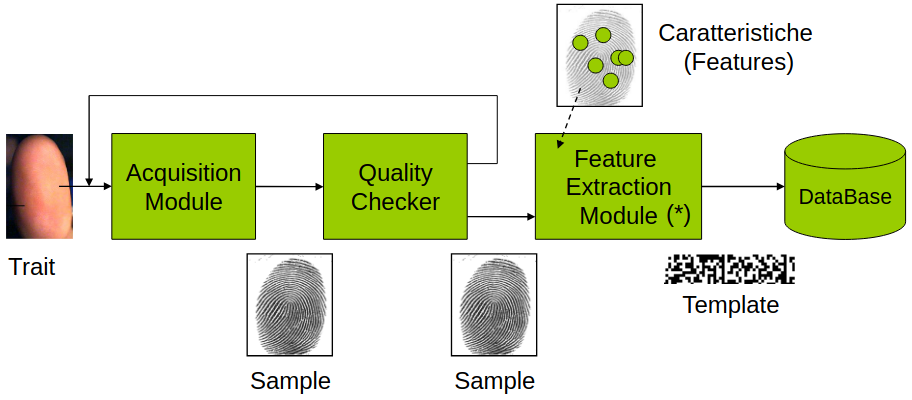
\includegraphics[width=0.95\linewidth]{images/enrollment-gen.png}
    \caption{Enrollment: (template) --$>$ DB}
    \label{fig:enroll-gen}
\end{figure}

\begin{figure}[ht]
    \centering
    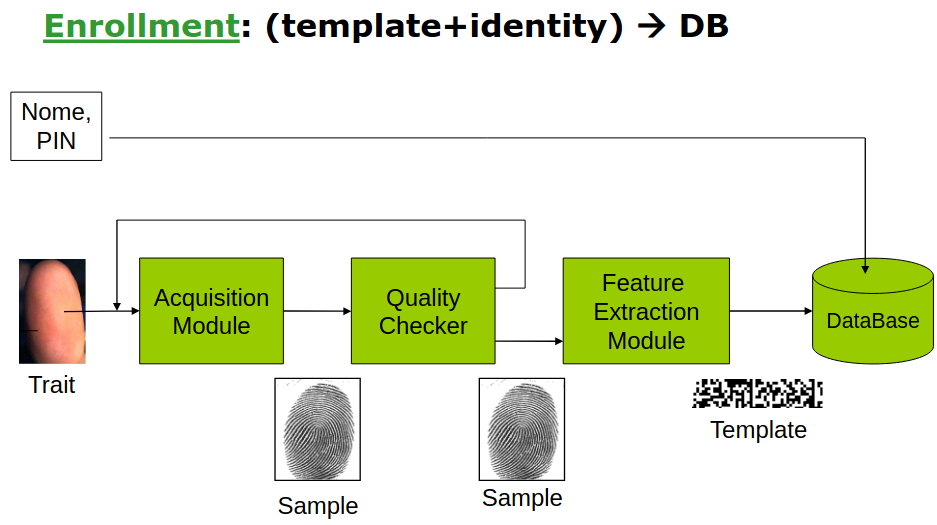
\includegraphics[width=0.95\linewidth]{images/enrollment-gen-id.png}
    \caption{(template + identity) --$>$ DB}
    \label{fig:enroll-gen-id}
\end{figure}

\newpage

\subsection{Verification usando un DB}

\begin{figure}[ht]
    \centering
    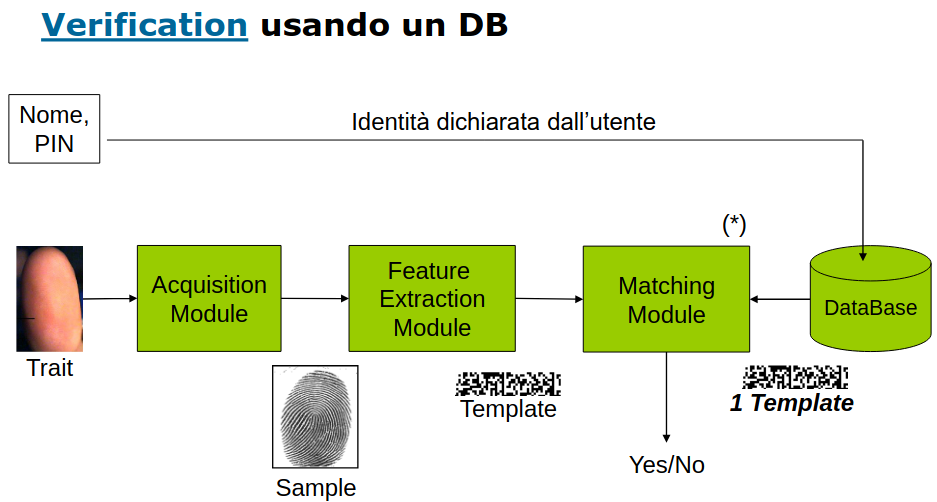
\includegraphics[width=0.95\linewidth]{images/verification-gen.png}
    \caption{Verification usando un DB}
    \label{fig:verification-gen}
\end{figure}

\newpage
\subsection{Identification}

\begin{figure}[ht]
    \centering
    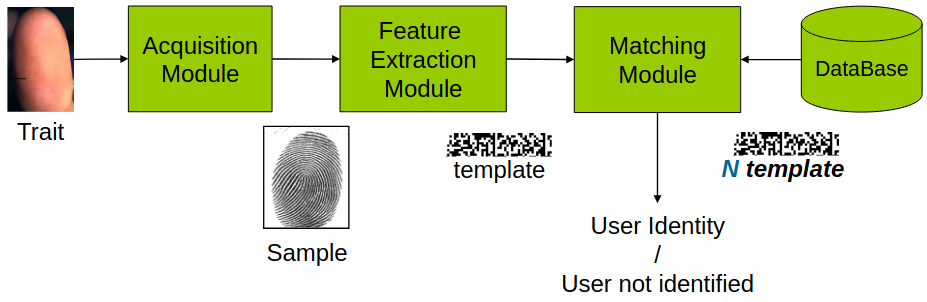
\includegraphics[width=0.95\linewidth]{images/identification-gen.png}
    \caption{Identification}
    \label{fig:id-gen}
\end{figure}

\section{Struttura per documenti biometrici}

\subsection{Fase di enrollment}

\begin{figure}[ht]
    \centering
    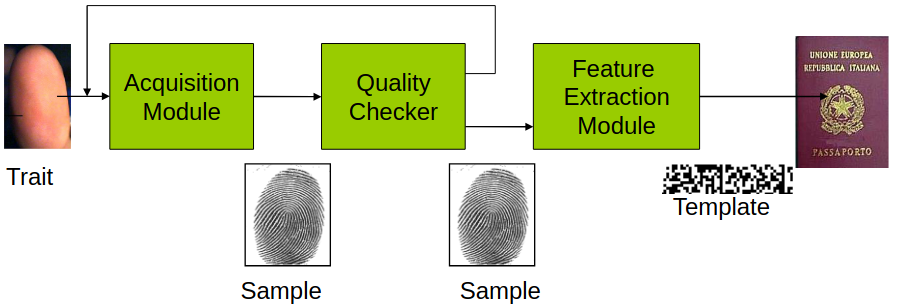
\includegraphics[width=0.95\linewidth]{images/enroll-doc.png}
    \caption{(template) --$>$ Documento}
    \label{fig:enroll-doc}
\end{figure}

\newpage
\subsection{Verification (con documento biometrico)}

\begin{figure}[ht]
    \centering
    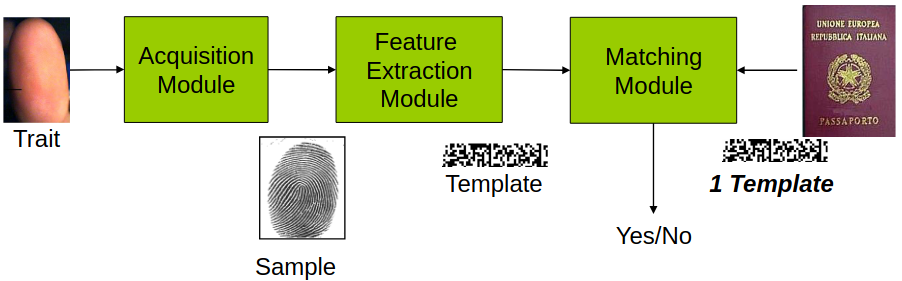
\includegraphics[width=0.95\linewidth]{images/verification-doc.png}
    \caption{Verification con documento biometrico}
    \label{fig:enter-label}
\end{figure}

\section{Struttura dei sistemi multimodali}

\begin{figure}[ht]
    \centering
    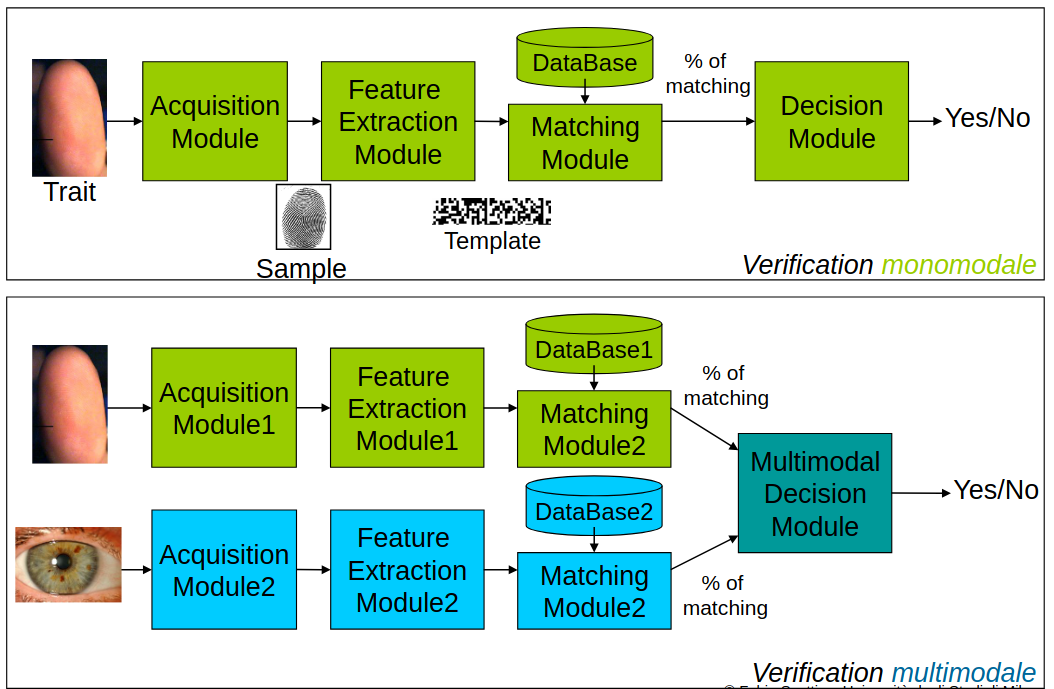
\includegraphics[width=0.95\linewidth]{images/multimodali.png}
    \caption{Confronto tra la struttura di un sistema monomodale e multimodale}
    \label{fig:multimodal}
\end{figure}

\newpage
\section{Struttura dei sistemi biometrici distribuiti}

Il termine “distribuito” si riferisce ad un sistema biometrico quando i moduli componenti sono separati e collegati in rete.
Piuttosto raro quando si parla di sistemi di autenticazione; è invece comune quando si parla di sistemi di identificazione di grosse dimensioni. 


\noindent Solitamente è il modulo dei database ad essere separato dai terminali.
\begin{figure}[ht]
    \centering
    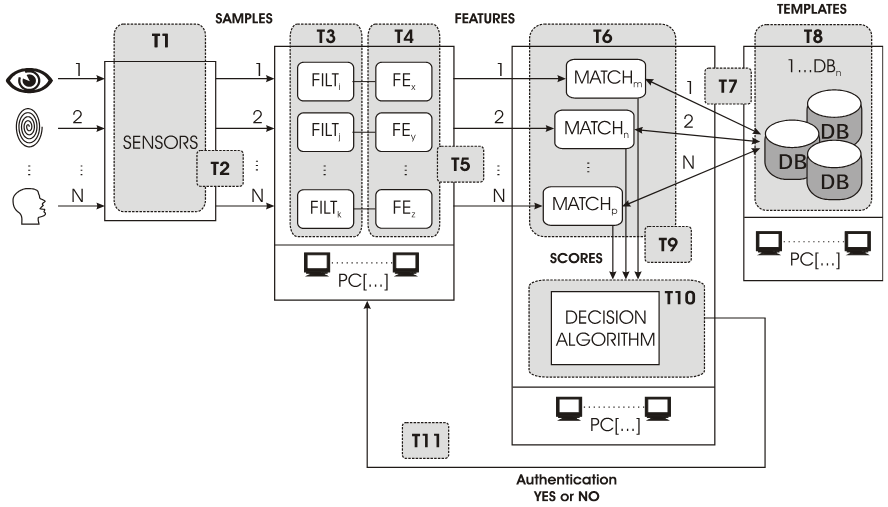
\includegraphics[width=0.95\linewidth]{images/distributed.png}
    \caption{Struttura di un sistema biometrico distribuito}
    \label{fig:distr}
\end{figure}

\section{Sistemi biometrici on card}
Il termine on card si riferisce al fatto che il template biometrico risiede su una smart card.



\chapter{Aspetti analitici di un sistema biometrico}

\section{Variabilità intraclasse}

Si intende la variazione del \textbf{sample} o delle \textbf{feature} dello stesso individuo tra acquisizioni effettuate in istanti di tempo diversi.
Può essere dovuto a:
\begin{itemize}
    \item effetti casuali (rumore del dispositivo)
    \item varizioni dello sfondo
    \item variazioni del tratto (invecchiamento, posizione, espressioni, ecc.)
\end{itemize}

\section{Similitudine interclasse}

Particolare vicinanza dei \textbf{sample} o delle \textbf{feature} acquisiti da individui diversi.





\chapter{Regole Generali di Progettazione}

\section{Acquisizione del tratto}

Analizziamo i metodi per \textbf{progettare} ed eventualmente \textbf{migliorare} il modulo di acquisizione.

\noindent L'acquisizione di una informazione rilevante \textbf{è un processo critico} e non sempre adeguatamente studiato.

\noindent La cura nel processo di acquisizione \textbf{influenza pesantemente l'accuratezza} finale del sistema.

Il processo di acquisizione si divide in \textbf{due fasi:}
\begin{itemize}
    \item \textbf{Valutazione della qualità:} controllo automatico sulla correttezza dei dati in ingresso coerentemente alle successive elaborazioni
    \item \textbf{Segmentazione:} separazione dei dati in ingresso nell'oggetto di interesse (foreground) e nello sfondo/informazione non rilevante (background)
\end{itemize}

\subsubsection{Estrarre molte informazioni}

È buona prassi cercare di estrarre maggiori informazioni possibili per migliorare le performance del sistema biometrico.
\begin{itemize}
    \item \textbf{Acquisire anche il contesto} attorno al sample; permette di trovare meglio il vero volto per sottrazione di frame senza elaborazioni troppo complesse
    \item \textbf{Evitare sul nascere di fare cattive acquisizioni} per non dover richiedere il sample (ad esempio, controllare se il soggetto è in movimento o alla distanza corretta prima di elaborare il frame)
\end{itemize}

\subsection{Controllo della qualità}

Dopo l'acquisizione molti sistemi attuano un controllo automatico della qualità del tratto rilevato per evitare problemi di funzionamento.

\noindent I sistemi di controllo della qualità producono un \textbf{indice di qualità} del sample acquisito:
\begin{itemize}
    \item se l'indice di qualità è sufficientemente alto si prosegue
    \item altrimenti si torna ad acquisire un altro sample
\end{itemize}

\noindent Il concetto di base è semplice, ma la progettazione e realizzazione dell'indice di qualità non lo è; alcuni punti sono che:
\begin{itemize}
    \item non sempre esiste un \textbf{modello rigoroso e realistico} della misura in ingresso da usare per calcolare l'indice; ad esempio, se potessimo definire come dovrebbe essere un'immagine ottimale di un'impronta, potremmo esprime l'indice di qualità come la "distanza" dell'immagine in ingresso da quella ottima
    \item non sempre esistono \textbf{metriche rigorose e robuste} per misurare la distanza del sample in ingresso con il riferimento ottimale
\end{itemize}

\subsubsection{Signal/Image enhancement}
In alcuni casi non è possibile rifiutare un sample perché il suo indice di qualità è basso (ad esempio database giudiziari); in questo caso, il sistema cerca di estrarre le informazioni (foreground) dal rumore (background) in modo tale da far funzionare il resto della catena di moduli del sistema.

Solitamente questa fase è ad alta complessità computazionale. Può generare i cosidetti \textbf{artefatti}; ad esempio, data un'impronta rumorosa genere delle minuzie che non erano presenti nell'immagine originale.

\section{Rappresentazione}

Un'acquisizione di un sistema non elaborata, chiamata sample, è:
\begin{itemize}
    \item \textbf{non invariante} rispetto al momento dell'acquisizione
    \item \textbf{non discriminatoria} (sono tutte diverse)
\end{itemize}

\noindent In un sistema biometrico occorre \textbf{studiare come rappresentare al meglio l'informazione} per rispondere 
alla domanda: \textit{"Quale rappresentazione machine-readable cattura \textbf{completamente} l'informazione \textbf{invariante} e \textbf{discriminatoria} 
della misura in ingresso?}

\noindent Il problema della rappresentazione consiste nel determinare uno spazio di misura che sia:
\begin{itemize}
    \item \textbf{invariante} (meno variante) rispetto ad acquisizioni dello stesso individuo
    \item che si \textbf{differinzi massivamente} dalla acquisizioni di individui diversi
\end{itemize}
In altre parole, si può dire che la rappresentazione deve fornire:
\begin{itemize}
    \item \textbf{alta variabilità interclasse} (io diverso da tutti gli altri)
    \item \textbf{bassa variabilità intraclasse} (io simile a me stesso nei miei sample)
\end{itemize}

\begin{figure}[ht]
    \centering
    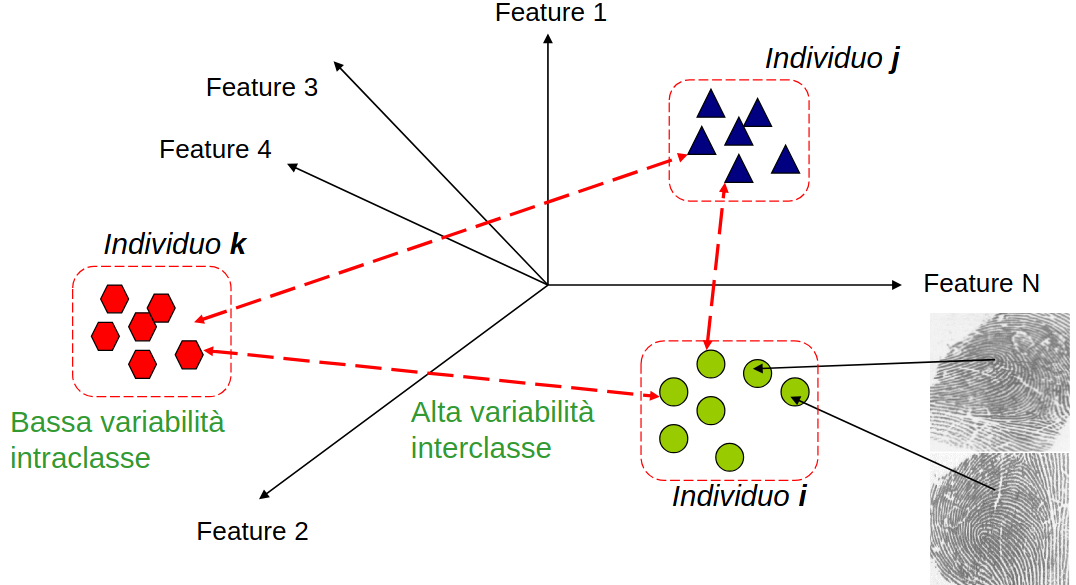
\includegraphics[width=1\linewidth]{images/rappresentazione.png}
    \caption{Visualizzazione del problema della
    rappresentazione in un spazio delle features
    N-dimensionale}
    \label{fig:rappr}
\end{figure}

\noindent Il problema della rappresentazione si suddivide in:
\begin{itemize}
    \item rappresentazione del sample
    \item estrazione delle caratteristiche
    \item rappresentazione del template
\end{itemize}

\subsection{Rappresentazione del sample}

Si riferisce alle caratteristiche tecniche del processo di acquisizione e memorizzazione del sample.
Varia a seconda del tratto biometrico, ci si riferisce a questi dati come \textbf{\textit{raw data}}.

\subsection{Estrazione di caratteristiche}

L'estrazione delle caratteristiche impatta sul modulo evidenziato
presente sia in fase di enrollment che di verification/identification.

\begin{figure}[ht]
    \centering
    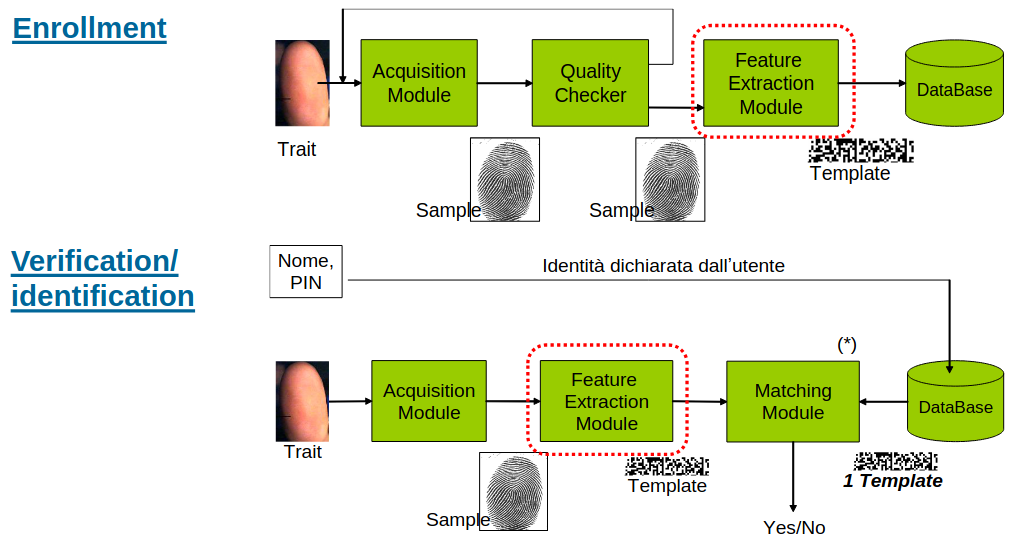
\includegraphics[width=1\linewidth]{images/estrazione.png}
    \caption{Impatto dell'estrazione delle caratterisiche}
\end{figure}

Avendo i dati raw provenienti dalle misurazioni occorre ora \textbf{estrarne la rappresentazione nello spazio delle caratteristiche.}
Questo non è mai un problema semplice, specialmente con dati rumorosi.

\noindent Può essere fatta in maniera manuale da un operatore oppure utilizzando un sistema automatico; \textbf{lo spazio delle 
caratteristiche di un sistema automatico tende ad essere diverso} da quello di un sistema con estrazione manuale.

\section{Matching}

Il matching impatta sul modulo evidenziato solo nella fase di verification\\/identification.

\begin{figure}[ht]
    \centering
    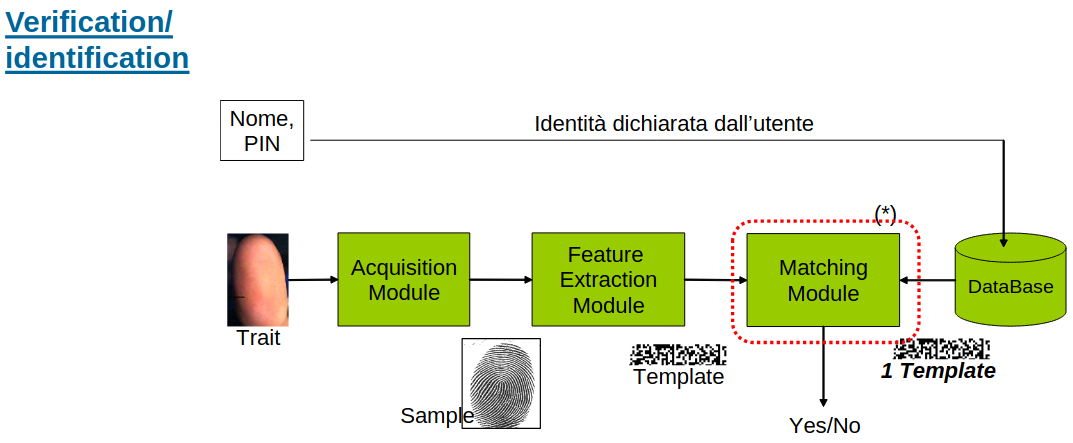
\includegraphics[width=1\linewidth]{images/matching.png}
    \caption{Impatto del matching}
\end{figure}

\section{Ricerca ed organizzazione dei DB biometrici}

\subsubsection{Scalabilità}

I sistemi che devono gestire una grande quantità di
identità dovrebbero essere in grado di operare
efficacemente quando il numero di utenti registrati nel DB
aumenta.

\noindent L'introduzione della biometria in un sistema di identificazione di grandi dimensioni produce dei vantaggi:
\begin{itemize}
    \item non soffrono del problema della produzione e del rinnovo dei documenti di identità
    \item sono competitivi in termini di costo e mantenimento
\end{itemize}

\subsection{Organizzazione del DB (indexing) e tasso di prenetazione nel DB}

L’obiettivo di gestire efficacemente la complessità delle
ricerche rispetto all’incremento del numero di template nel
DB del sistema può essere raggiunto solo con una attenta
organizzazione dei DB (indexing); un DB organizzato permette di non confrontare un
template in ingresso con tutti i template nel DB ma solo
con quelli contenuti in una partizione.

\begin{figure}[ht]
    \centering
    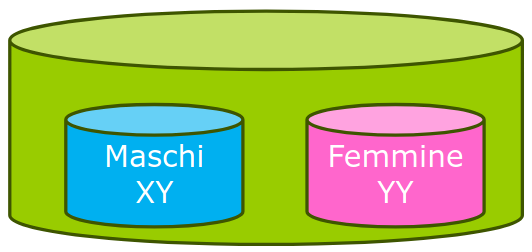
\includegraphics[width=0.75\linewidth]{images/indexing.png}
    \caption{Esempio di indexing}
\end{figure}

\noindent In generale si può definire il tasso di penetrazione come la
percentuale del database totale da esaminare in media per
ogni ricerca. Più basso è il tasso di penetrazione, più
efficiente è il sistema.

\noindent Tuttavia, per i sistemi biometrici serve fare un distinguo: 

\noindent \textit{\textbf{la proporzione attesa dei template da cercare su tutti i campioni di input secondo
la regola che la ricerca prosegue attraverso l'intera partizione, indipendentemente
dal fatto che venga trovata una corrispondenza o meno}}.

\subsection{Binning}

Per giovare delle partizioni del DB occorre disporre di un
\textbf{algoritmo automatico molto robusto} per la classificazione
dei template; quando il DB viene creato, i template vengono disposti nelle partizioni (\textbf{\textit{bins}}).

\begin{figure}[ht]
    \centering
    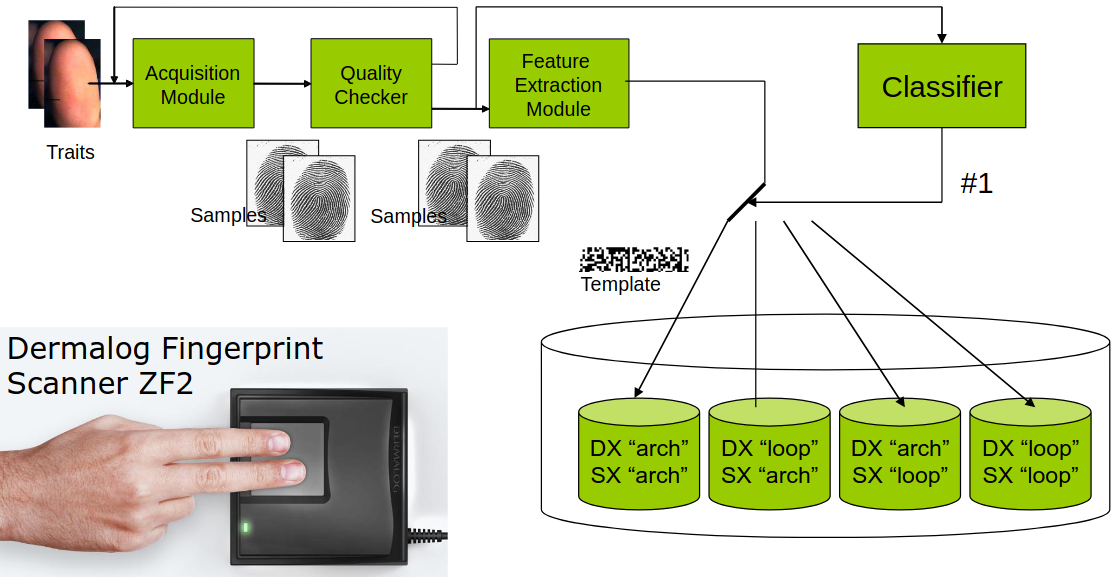
\includegraphics[width=1\linewidth]{images/binning.png}
    \caption{Esempio di suddivisioni in bins di un DB}
\end{figure}

\subsubsection{Calcolo del numero di bin ottimale}

Se ho \textbf{N} impronte disitnguibili (indice, medio...) tutte divisibili \textbf{M} tipi (arch, whorl, ...), allora 
numero migliore di bin è = \textbf{$M^N$}.

\subsubsection{Binning error}

I  problemi nascono quando un individuo presenta i propri
tratti biometrici al sistema e l’algoritmo di classificazione
del tratto sbaglia il bin (binning error); se l'indivduo era registrato nel DB, probabilmente non si avrà un match in quanto i template che matchano sono in un bin differente.

\newpage

\subsubsection{Calcolo del binning error}

Definiamo:

\textit{Binning error} = \textbf{Prob(}fare almeno 1 errore\textbf{)}

\textit{p} = \textbf{Prob(}sbagliare una classificazione\textbf{)} \\\\
Allora:

\textit{Binning error} = \textbf{Prob(}fare almeno 1 errore\textbf{)}

= 1 - \textbf{Prob(}0 errori\textbf{)}

= 1 - $(1-p)*(1-p)$

= 1 - $(p^2-2p+1)$

= $2p - p^2$ = 2p - \textit{molto poco (se p è piccola)}
\\
\\
Ne consegue che:

\textbf{Binning error} $\rightarrow$ \textbf{circa} $N*p$ \textbf{se si usano N impronte} se:

- \textit{p} è piccola (vero)

- classi distribuite (simile numero di impronte nei bin, vero)\\\\
Se si \textbf{abbassano il numero delle classi:}
\begin{itemize}
    \item \textbf{\textcolor{red}{Si alza il P.R. $\rightarrow$ si abbassa la qualità del P.R. ottenibile}}
    \item \textbf{\textcolor{green}{Si abbassa l'errore di classificazione}}
\end{itemize}


\chapter{Introduzione alla misura dei parametri}
Nel caso dei sistemi biometrici non è banale rispondere alla domanda: \textit{\textbf{
    "qual è il tasso di errore di verifica/identificazione?"
}}

\noindent Per descrivere le performance del sistema è necessario disporre di \textbf{un insieme di dati} e \textbf{curve di funzionamento};
per questo motivo diventa difficile comparare due sistemi in quanto non basta confrontare 2 numeri.

\subsubsection{Genuini ed impostori}

Si impiegano i termini:
\begin{itemize}
    \item \textbf{genuino} per indicare un individuo che accede al sistema e ha titolo per farlo
    \item \textbf{impostore} per chi prova ad accedere senza averne titolo
\end{itemize}

\noindent La formulazione del problema risulterà diversa a seconda che il sistema funzioni in \textbf{verification} o \textbf{identification}.

\newpage

\section{Verifica e Identificazione}

\subsection{Verifica}

\textit{"tu sei chi dici di essere?"}
\\
Il problema in questo caso si riconduce ad un caso di classificazione binaria.

\subsubsection{Problema della verifica}

Dato in ingresso un insieme di caratteristiche $X_Q$ e la dichiarata identità $I$,
occorre determinare se $(I, X_Q)$ appartiene a $w_1$ o $w_2$, dove:
\begin{itemize}
    \item $w_1$ indica che la richiesta è vera (utente genuino)
    \item $w_2$ indica che la richiesta è falsa (un impostore)
\end{itemize}

\noindent Tipicamente, le caratteristiche $X_Q$ vengono controllate con le caratteristiche $X_I$ (il template associato alla identità $I$).

\subsubsection{Regola di decisione per la verifica}

Si tratta di una comparazione con soglia:
\begin{figure}[ht]
    \centering
    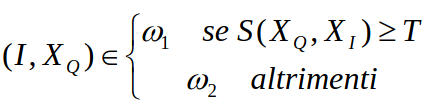
\includegraphics[width=0.5\linewidth]{images/regola-verifica.png}
\end{figure}

\noindent Dove:
\begin{itemize}
    \item $S$ è la funzione che misura la similitudine tra $X_Q$ e $X_I$
    \item $T$ è la soglia prefissata
    \item $S(X_Q, X_I)$  prende il nome di \textbf{match score}
\end{itemize}

\subsection{Identificazione}
\textit{"il sistema controlla se i tuoi dati biometrici corrispondono
 ad un insieme di identità registrate"}

\subsubsection{Problema di identificazione}
Dato in ingresso un insieme di caratteristiche $X_Q$, determinare l'identità 
$I_k$, con $k \in \{1,2,3,...,M,M+1\}$ dove $I_1, I_2,...,I_M$ sono 
le M identità memorizzate nel sistema e $I_M+1$ rappresenta il \textbf{caso di reiezione}.

\noindent Nel caso di reiezione nessuna delle M identità registrate è sufficientemente simile al dato in ingresso.

\newpage

\subsubsection{Regola di decisione per l'identificazione}
Si tratta di M comparazioni con soglia con la seguente regola di decisione:
\begin{figure}[ht]
    \centering
    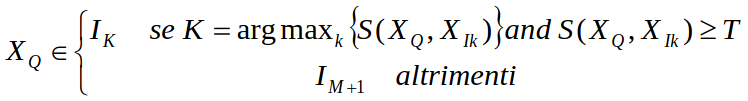
\includegraphics[width=1\linewidth]{images/regola-identificazione.png}
\end{figure}

\noindent Dove:
\begin{itemize}
    \item $X_Ik$ è il template corrispondente alla identità $I_k$
    \item $T$ è la soglia prefissata
    \item $S(X_Q, X_I)$ prende il nome di \textbf{match score}
\end{itemize}

In alcuni casi ci si riferisce ad una \textbf{misura della distanza} fra
$X_Q$ e $X_I$; una \textbf{grande distanza} fra i vettori di features porta ad un \textbf{basso match score}.

\section{Distanza tra template}

N template, provenienti dalla stessa persona ma acquisiti in tempi diversi,
NON sono \textbf{mai uguali}.

\noindent Esiste sempre una distanza nello spazio delle features che separa i template anche della 
stessa persona (rumore, posa del soggetto, illuminazione, condizione ambientiali, \dots)

\noindent Questa comporta che \textbf{la soglia $T$ non può esser arbitrariamente abbassata}, altrimenti 
nessuno sarebbe identificato.

\noindent Se si riscontrasse una \textbf{distanza nulla} fra $X_Q$ e $X_I$ (quindi $S(X_Q, X_I) = max$), probabilmente 
saremmo di fronte ad un \textbf{replay attack}: una copia illecita di un template memorizzato che viene 
riproposto per frodare un sistema.

\subsubsection{Genuini ed impostori}

Si parla di \textbf{\textcolor{green}{genuine score}} quando si confrontano le distanze tra i template
dello stesso individuo.

\noindent Si  parla di \textbf{\textcolor{red}{impostor score}} quando si confrontano le distanze tra i template 
di indivdui diversi.

\newpage

\subsection{Distribuzioni dei match score}

\begin{figure}[ht]
    \centering
    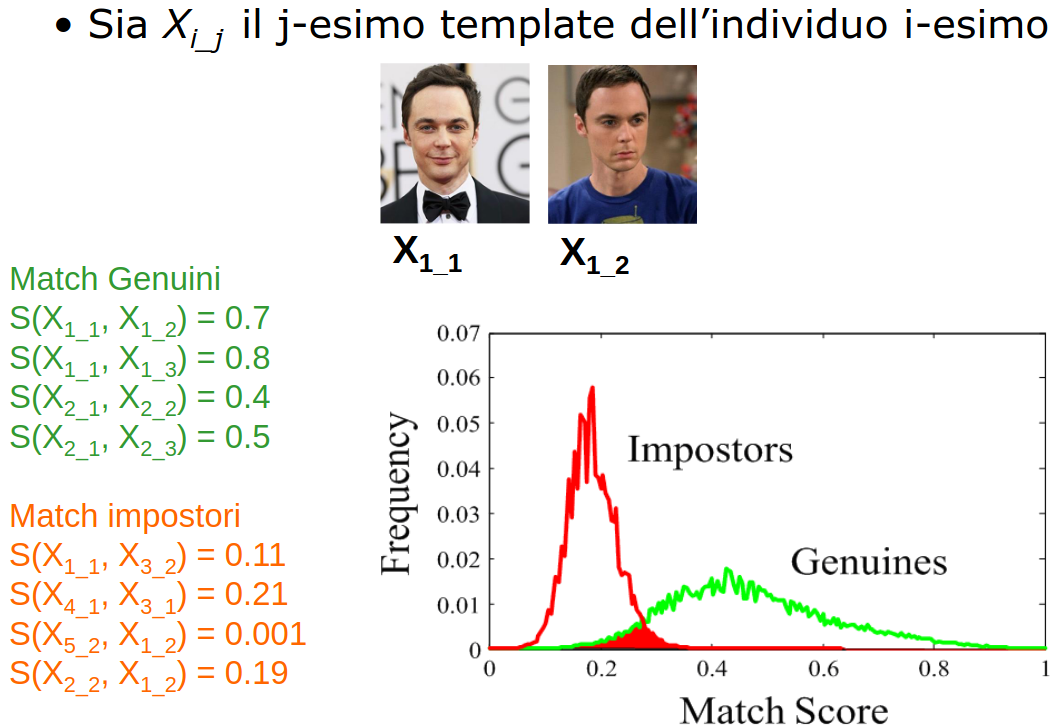
\includegraphics[width=1\linewidth]{images/distr-matchscore.png}
\end{figure}

\section{False Match e False Non-Match}

\begin{itemize}
    \item \textbf{False Match:} \textit{il ladro entra in casa perché il sistema lo 
    ha scambiato per noi;} \textbf{$impostorScore > T$}
    \item \textbf{False Non-Match:} \textit{non entrate in casa perché il sistema ritiene che il template non assomigli
    abbastanza a quello/i registrati;} \textbf{$genuineScore < T$}
\end{itemize}

\subsection{FM Rate, FNM Rate}

Supponiamo di poter variare la soglia e di fissarla a un valore $T$ in mezzo fra il picco
degli impostori e quello dei genuini. Notiamo che:
\begin{itemize}
    \item un certo numero di persone appartenenti al gruppo dei \textbf{\textcolor{green}{genuini}} 
    sono \textbf{sotto la soglia T}; non saranno autorizzati e daranno errore di
    False Non-Match (FNM).

    \textit{FNMR(T) = FNM(T) / numGenuini}
    \item una parte degli \textbf{\textcolor{red}{impostori}} hanno valori di match
    \textbf{sopra la soglia T}; saranno autorizzati e daranno errori di False Match (FM).

    \textit{FMR(T) = FM(T) / numImpostori}
\end{itemize}

\begin{figure}[ht]
    \centering
    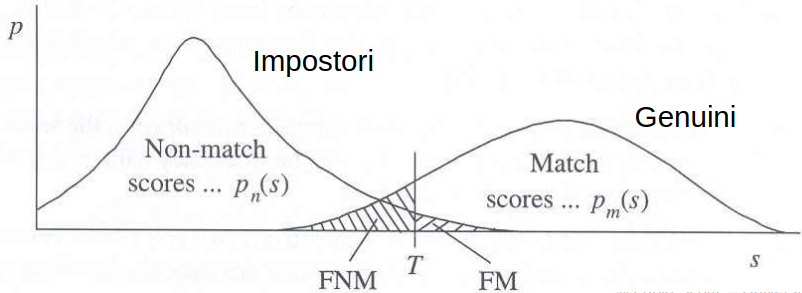
\includegraphics[width=1\linewidth]{images/rate.png}
    \caption{FNM e FM}
    \label{fig:rate}
\end{figure}

\noindent Il funzionamento di un sistema biometrico dal punto di vista degli errori commessi 
è descritto dai tassi \textit{FMR(T)} e \textit{FNMR(T)} per tutti i valori della soglia.

\section{Decision Error Tradeoff (DET) e Receiver Operating Characteristic (ROC)}

\subsubsection{DET: Regioni di funzionamento}
Regolando la soglia T possiamo regolare il livello di sicurezza.

\begin{figure}[ht]
    \centering
    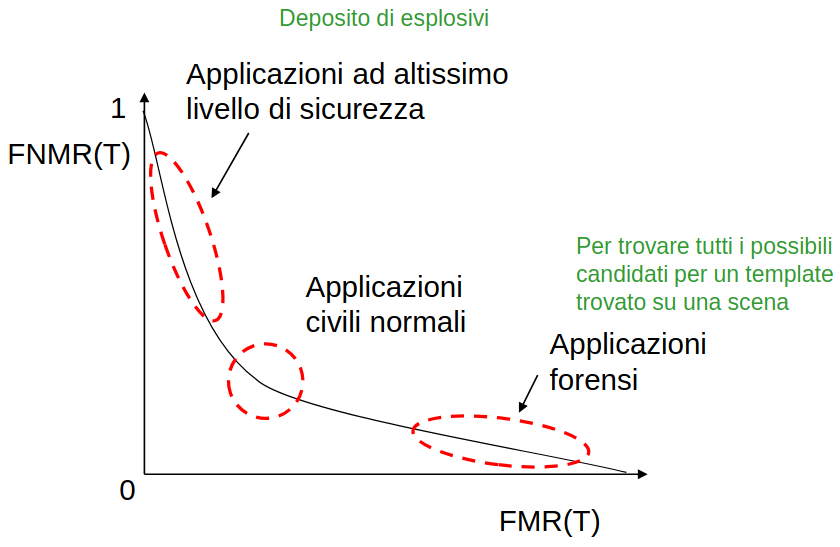
\includegraphics[width=1\linewidth]{images/det.png}
\end{figure}

\subsubsection{DET: Equal Error Rate}

L'EER è il tasso di errore corrispondente all'unico punto nel
quale si ha FNMR = FMR.

\noindent Si tratta dell'unico numero singolo che può riassumere il funzionamento del sistema.

\subsubsection{ROC = 1 - DET}

\textbf{La curva DET e ROC mostrano le stesse informazioni}.
La DET mette l'attenzione sul FNM (genuini che non entrano), mentre la ROC 
mette l'evidenza su 1 - FNM (quanti genuini riescono ad entrare).

\begin{figure}[ht]
    \centering
    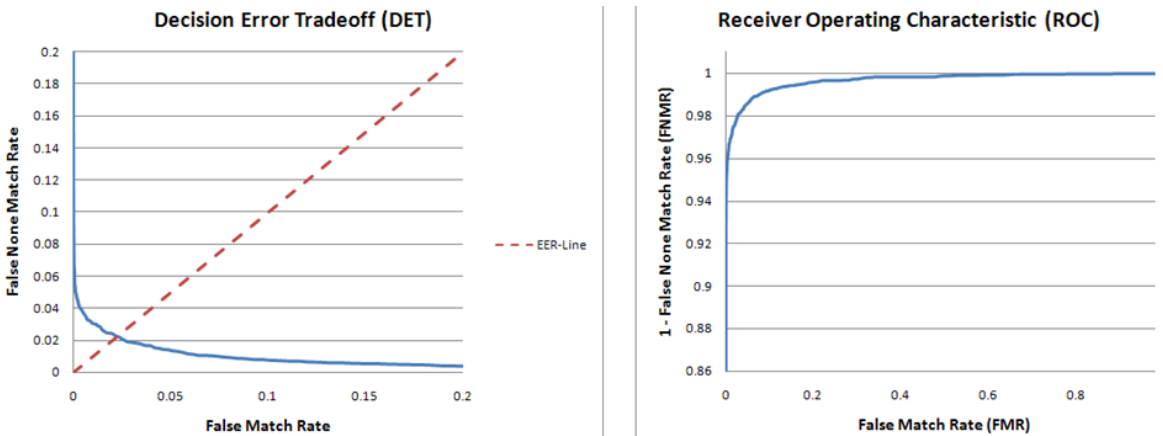
\includegraphics[width=1\linewidth]{images/det-roc.png}
    \caption{Curve DET e ROC}
\end{figure}

\section{Metodi statistici per la stima dei parametri in
un sistema biometrico}

\subsection{Che modello usiamo?}

Chiariamo il concetto di \textbf{Prova/Esperimento di Bernoulli:}
\begin{enumerate}
    \item ad ogni singola prova si hanno solo due esiti possibili
    \begin{itemize}
        \item successo (1)
        \item insuccesso (0)
    \end{itemize}
    \item La probabilità \textbf{\textit{p}} dell'evento 'successo' è costante
    \item i risultati delle prove sono \textbf{indipendenti}
\end{enumerate}

\noindent Date due impronte il SB in autenticazione mostra un tasso di errori stimabile e fissato \textit{\textbf{p}}.

\noindent L'evento che il SB sbagli una autenticazione è un \textbf{esperimento/prova di Bernoulli}.

\noindent Un SB usato in identificazione (1:N) si può modellizzare come un N prove di Bernoulli, 
ovvero un \textbf{processo di Bernoulli}.

\subsection{Regola dei 3}

\textit{"qual è il tasso di errore più basso p che può essere stimato con un esperimento
di comparazione di N campioni indipendenti?"}

\noindent Se abbiamo un sistema che commette 0 errori su N prove non dobbiamo pensare di
avere un sistema con $p=0$, ma con il 95\% di confidenza abbiamo un sistema
che ha $p \approx 3/N$.

\subsubsection{Esempio}

Se faccio 300 prove e ho 0 errori, allora posso dire con confidenza del 95\% che
il sistema ha un tasso di errore stimato del $p \approx 3/N = 3/100 = 1\%$

\subsection{Regola dei 30}

La regola dei 30 è utilizzata per determinare la larghezza del campione biometrico in questo modo:
\begin{itemize}
    \item per essere sicuro con intervallo di confidenza del 90\% che il tasso di errore \textbf{vero}
    sia tra il $\pm 30 \%$ del tasso di errore \textbf{osservato}, ci devono essere almeno 30 errori.    
\end{itemize}

\subsubsection{Esempio}
Se abbiamo 30 FNM in 3000 comparazioni, possiamo dire (con intervallo di 
confidenza del 90\%) che l'errore vero sia tra $0,7\%$ e $1,3\%$.










\end{document}